\documentclass{report}

%\usepackage{fullpage}
%\usepackage[skip=4pt]{caption} % ``skip'' sets the spacing between the figure and the caption.
\usepackage{tikz}
\usetikzlibrary{positioning}
\usepackage{xcolor}

%\usepackage[hidelinks]{hyperref}   % Make the cross references clickable hyperlinks
%\usepackage[bottom]{footmisc} % Prevents the table going below the footnote

% Set up page formatting
%\usepackage{fancyhdr} % Used for every page footer and title.
%\pagestyle{fancy}
%\fancyhf{} % Clears both the header and footer
%\renewcommand{\headrulewidth}{0pt} % Eliminates line at the top of the page.
%\fancyfoot[LO]{CMPS242 \textendash{} Homework \#5} % Left
%\fancyfoot[CO]{\thepage} % Center
%\fancyfoot[RO]{Sherman \& Hammoudeh} %Right

\renewcommand\thesection{\arabic{section}} % Prevent chapter number in section number.

% Change interline spacing.
\renewcommand{\baselinestretch}{1.1}
\newcommand{\norm}[1]{\left\lVert#1\right\rVert}


\title{\textbf{CMPS242 Homework \#5 \textendash{} Neural Network Tweet Classification}}
\author{Benjamin Sherman \\~\\ \& \\~\\ Zayd Hammoudeh}


\begin{document}
  \maketitle
  
  \section{Homework Objective}
  \section{Feed-Forward Neural Network Structure}
  
  \begin{figure}
    \tikzset{
      sigmoid/.style={path picture= {
          \begin{scope}[x=1pt,y=10pt]
            \draw plot[domain=-6:6] (\x,{1/(1 + exp(-\x))-0.5});
          \end{scope}
        }
      },
      relu/.style={path picture= {
          \begin{scope}[x=1pt,y=1pt]
            \draw plot[thick,domain=-8:0] (\x,{-3});
            \draw plot[ultra thin,domain=0:8] (\x,{-3+\x});
          \end{scope}
        }
      },
      every neuron/.style={
        circle,
        draw,
        minimum size=1cm,
      },
      neuron filled/.style={
        every neuron,
        fill=gray!10
      },
      neuron bias/.style={
        every neuron,
        font={Bias}
      },
      neuron output/.style={
        every neuron,
        sigmoid
      },
      neuron hidden/.style={
        every neuron,
        relu
      },
      neuron missing/.style={
        draw=none, 
        scale=4,
        text height=0.3cm,
        execute at begin node=\color{black}$\vdots$
      },
    }
  
    
    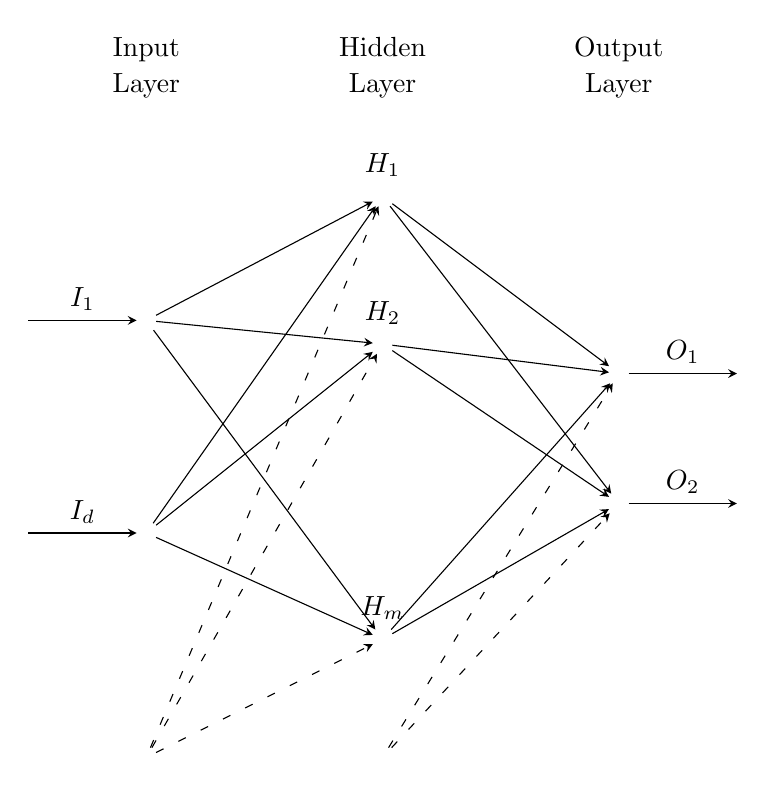
\begin{tikzpicture}[x=1.5cm, y=1.5cm, >=stealth]
      \foreach \m/\l [count=\y] in {1,missing,2}
        \node [every neuron/.try, neuron \m/.try] (input-\m) at (0,1.1-\y*0.9) {};
      
      %\foreach \m [count=\y] in {1,2,missing,3}
      %  \node [neuron hidden/.try, neuron \m/.try ] (hidden-\m) at (2,2.5-\y*1.25) {};
      \node [neuron hidden/.try, neuron 1/.try ] (hidden-1) at (2,2.5-1*1.25) {};
      \node [neuron hidden/.try, neuron 2/.try ] (hidden-2) at (2,2.5-2*1.25) {};
      \node [every neuron/.try, neuron missing/.try ] (hidden-missing) at (2,2.5-2.95*1.25) {};
      \node [neuron hidden/.try, neuron 3/.try ] (hidden-3) at (2,2.5-4*1.25) {};
      
      \foreach \m [count=\y] in {1,2}
        \node [neuron output/.try, neuron \m/.try ] (output-\m) at (4,0.85-\y*1.1) {};
      
      \foreach \m [count=\y] in {1,2}{
        \node [neuron filled/.try] (filled-\m) at (-2+2*\y,-3.5) {};
        \node [neuron bias/.try] (bias-\m) at (-2+2*\y,-3.5) {};
      }
      
      % Add the labels to the nodes
      \foreach \l [count=\i] in {1,d}
        \draw [<-] (input-\i) -- ++(-1,0)
        node [above, midway] {$I_\l$};
      
      \foreach \l [count=\i] in {1,2,m}
        \node [above] at (hidden-\i.north) {$H_\l$};
      
      \foreach \l [count=\i] in {1,2}
        \draw [->] (output-\i) -- ++(1,0)
        node [above, midway] {$O_\l$};
      
      % Draw the connecting arrows
      \foreach \i in {1,...,2}
        \foreach \j in {1,...,3}
          \draw [->] (input-\i) -- (hidden-\j);
      
      \foreach \i in {1,...,3}
        \foreach \j in {1,...,2}
          \draw [->] (hidden-\i) -- (output-\j);

      \foreach \i in {1,...,3}
        \draw [loosely dashed, ->] (bias-1) -- (hidden-\i);
      \foreach \i in {1,...,2}
        \draw [loosely dashed, ->] (bias-2) -- (output-\i);
          
      
      \foreach \l [count=\x from 0] in {Input, Hidden, Output}
      \node [align=center, above] at (\x*2,2) {\l \\ Layer};
    \end{tikzpicture} 
    \caption{Base Structure of Our Feed-Forward Network}\label{fig:feedForwardNet}
  \end{figure}
  
  The base structure of our feed forward network is shown in Figure~\ref{fig:feedForwardNet}.  The number of input nodes is dictated by the number of rows in the embedding matrix; as mentioned previously, $d=25$~in our experiments.  Likewise, the number of neurons in the hidden layer was~$m=256$. There were two output nodes (e.g., one for ``Donald Trump'' and the other for ``Hillary Clinton).  All nodes had their own bias input to improve performance.  
  
  Our final feed-forward network design used the rectified linear and sigmoid activation functions for the hidden and output layers respectively.
  
  
  \section{Extra Credit \#1: Bag of Words Model}
  
  In the ``bag of words'' model, each textual input, i.e., tweet, is transformed into an unordered set of words.  Hence, the contextual and word ordering information is discarded.  This approach removes any sequential relation in the data; hence, the LSTM added no specific value for training.  Hence, we removed the LSTM when performing this experiment and instead trained with just the embedding matrix and the feed-forward network. 
  
  Using the previously described neural-network structure, we were able to get 100\%~accuracy on the complete training set.  Likewise, we get an best-case test set of~\textbf{0.20070} using this approach.
  
  \section{Extra Credit \#2: Neural Network Experiments}
  
  Below are additional experiments we tried beyond the base requirements.  
  
  \subsection{Extra Credit \#2a: Hidden Layer Activation Functions}
  
  We experimented with three activation configurations for the hidden layer.  In addition to rectified linear, we also tried a ``pass-through'' activation where the 
  
  \subsection{Extra Credit \#2b: Additional Feed-Forward Hidden Layers}
  
   
\end{document}